\section{Power electronic components for current control}\label{BASICCSR:sec:PowerGeneral}

As the introduction suggest the main topic of the thesis is optimal current control. As such for reaching the desired optimum, the necessary actuators are needed for the task. For this, power electric converters are used, all of them based on a simple principle, namely they use controllable switches to set the required voltage level or the conducting current value, required on the load's end.

\subsection{Current source inverters}\label{BASICCSR:sec:CSI}

Single-phase inverter's operating principles are different in each converter. The main features of the different approaches are reviewed and presented in the following. Although these converters cover the low-power range, they are widely used in power supplies or single-phase supplies. For this thesis a domestic current source inverter is considered, which fits into this category.\\
A current source inverter is composed of capacitors, switches, and diodes, where an array of two switches is called inverter leg shown in Fig.\ref{BASICCSR:fig:SingleCSI}. The capacitors required to provide a neutral point, such that each capacitor maintains a constant voltage.

\begin{figure}[!ht]
        \centering
        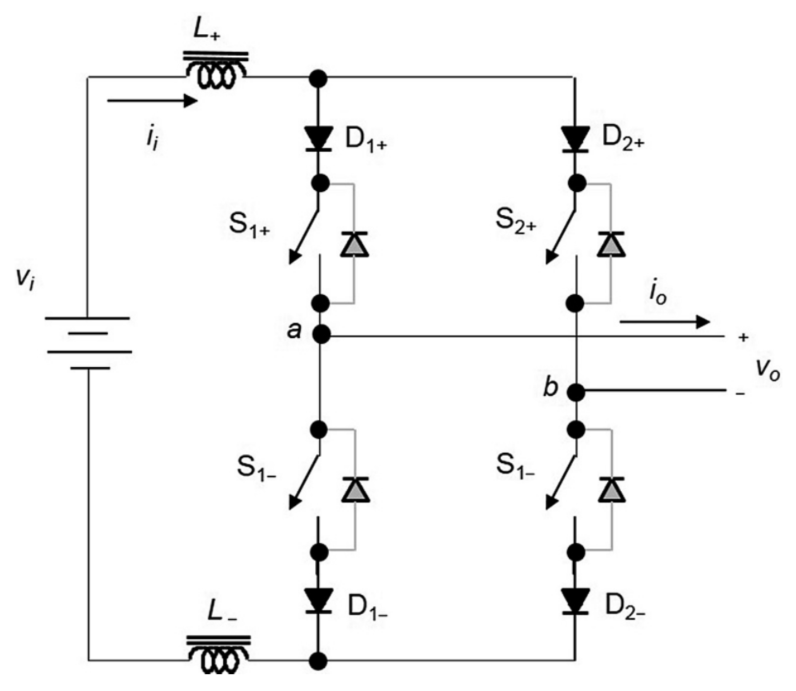
\includegraphics[width=0.6\textwidth]{EMPC_PNG_Pics/CurrentSourceInverter.png}
        \caption{Topology of a singly phase current source inverter, where $V_i$, and $V_o$ are the input and output voltages, $i_i$, and $i_o$ are the input and output currents respectively. $L_+$ and $L_-$ are current filter inductances, $S_{1+}$, $S_{2+}$, $D_{1+}$, and $D_{2+}$ are the higher switches (controlled IGBTs for instance) and diodes, and $S_{1-}$, $S_{2-}$, $D_{1-}$, and $D_{2-}$ are the lower switches and diodes respectively.}
        \label{BASICCSR:fig:SingleCSI}
    \end{figure}

The inductors required are large, such that the inductors
maintain a constant current $i_i$. Current-source topologies feature a low switching voltage gradient and reliable over-current or short-circuit protection. In order to operate properly the current-source inverter, we need to adhere to the following rules:
\begin{itemize}
\item Top or bottom switches of the different legs cannot be off simultaneously, because no current path is provided to the input inductors.
\item Diode must be placed in series with each switch, because a short circuit across the output voltage $V_o$ would be produced. If the commercial switch does not include anti- parallel diodes, then the circuit is already complete.
\item In practical implementation, an overlapping time must be considered in the control signals of the top or bottom switches of the different legs.
\end{itemize}

According to the previous rules, it should be noticed that all switches of the inverter leg can be turned on at the same time. This is not possible in voltage source inverters. There are four ($1^{st}$ to $4^{th}$) defined states of the switches and one not permitted switching state ($5^{th}$ state) as shown in Table \ref{BASICCSR:table:CSIstates}. The modulating technique should always ensure that at any instant, at least one of the top and bottom switch of the inverter legs is on, otherwise the inverter will be damaged.

% Please add the following required packages to your document preamble:
% \usepackage{multirow}
\begin{table}[h!]
\centering
\caption{Switching states of the current source inverter, where $V_{an}$, $V_{bn}$ are the $a$ and $b$ point's potential to ground.}
\begin{tabu}{|c|c|c|c|c|c|c|c|}
\hline
\multicolumn{4}{|c|}{Components conducting} & \multirow{2}{*}{State} & \multicolumn{3}{c|}{Output voltages}                \\ \cline{1-4} \cline{6-8}
$S_{1+}$       & $S_{2+}$       & $S_{1-}$      & $S_{2-}$      &                        & $V_{an}$              & $V_{bn}$              & $V_{o}$           \\ \tabucline[2pt]{-}
1         & 0         & 0        & 1        & 1                      & $V_{i}/2$            & -$V_{i}/2$           & $V_{i}$           \\ \hline
0         & 1         & 1        & 0        & 2                      & -$V_{i}/2$          & $V_{i}/2$            & -$V_{i}$          \\ \hline
1         & 1         & 0        & 0        & 3                      & $V_{i}/2$             & $V_{i}/2$            & 0             \\ \hline
0         & 0         & 1        & 1        & 4                      & -$V_{i}/2$           & -$V_{i}/2$          & 0             \\ \hline
0         & -         & 0        & -        & \multirow{2}{*}{5}     & \multicolumn{3}{c|}{\multirow{2}{*}{Not permitted}} \\ \cline{1-4}
-         & 0         & -        & 0        &                        & \multicolumn{3}{c|}{}                               \\ \hline
\end{tabu}

\label{BASICCSR:table:CSIstates}
\end{table}

The ideal waveforms are shown in Fig.\ref{BASICCSR:fig:CSIwave_All}.

\begin{figure}[h!]
                \centering
                \begin{subfigure}[b]{0.9\textwidth}
                    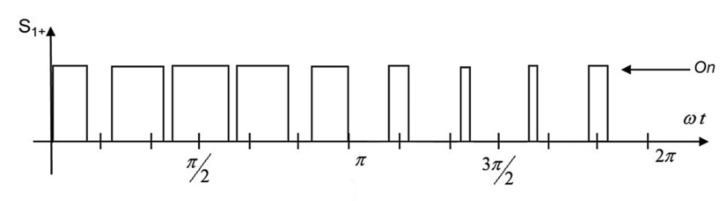
\includegraphics[width=\textwidth]{EMPC_PNG_Pics/CSIwaves_A.png}
                    \caption{\centering The state of switch $S_{1+}$.}
                    \label{BASICCSR:fig:CSIwave_A}
                \end{subfigure}
                ~ %add desired spacing between images, e. g. ~, \quad, \qquad, \hfill etc.
                  %(or a blank line to force the subfigure onto a new line)
                \begin{subfigure}[b]{0.9\textwidth}
                    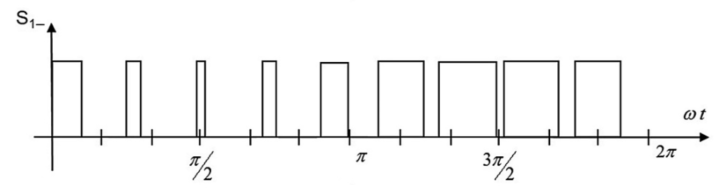
\includegraphics[width=\textwidth]{EMPC_PNG_Pics/CSIwaves_B.png}
                    \caption{\centering The state of switch $S_{2+}$..}
                    \label{BASICCSR:fig:CSIwave_B}
                \end{subfigure}
								 ~ %add desired spacing between images, e. g. ~, \quad, \qquad, \hfill etc.
                  %(or a blank line to force the subfigure onto a new line)
                \begin{subfigure}[b]{0.9\textwidth}
                    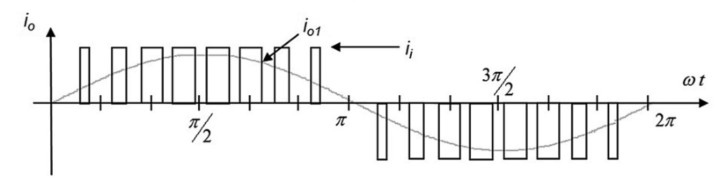
\includegraphics[width=\textwidth]{EMPC_PNG_Pics/CSIwaves_C.png}
                    \caption{\centering AC output current.}
                    \label{BASICCSR:fig:CSIwave_C}
                \end{subfigure}

                \caption{The CSI, ideal waveforms as the result of the modulation.}
                \label{BASICCSR:fig:CSIwave_All}
            \end{figure}

The states for the switches are defined by the modulating technique, which in this case is a carrier-based PWM, but unipolar output is considered. For the CSIs, different output filters may be employed, in order to provide the fundamental component of the output waveform. Depending on the application, it would be desirable to provide a voltage or current output.

\subsection{Galvanic decoupled bi-directional DC-DC converters}\label{BASICCSR:sec:DCDC}

In this section a basic galvanic decoupled voltage source DC-DC converter shall be presented. In many DC power supplies, a galvanic isolation between the DC or AC input and the DC output is required for safety and reliability. An economical mean of achieving such an isolation is to employ a transformer version of a DC-DC converter. High-frequency transformers are of small size and weight and provide high efficiency. Their turns ratio can be used to additionally adjust the output voltage level. Generally, electric power generated by renewable energy sources is unstable in nature, thus producing an unwanted effect on the utility grid. This fact motivates research on energy storage and quality systems to smooth out active-power flow.\\
On the converter Fig.\ref{BASICCSR:fig:DCDCGalvanic} has two symmetrical single-phase voltage-source full-bridge converters, allowing a bi-directional power flow. Thanks to advancement in power device technology over the last decade the DC-DC devices are able to operate at an efficiency as high as $\approx97\%$ by using the latest trench-gate IGBTs. Therefore this topology has become a promising candidate as a power electronic interface for an energy storage and renewable system \cite{kheraluwala1992performance} \cite{inoue2007bidirectional}.


\begin{figure}[!ht]
        \centering
        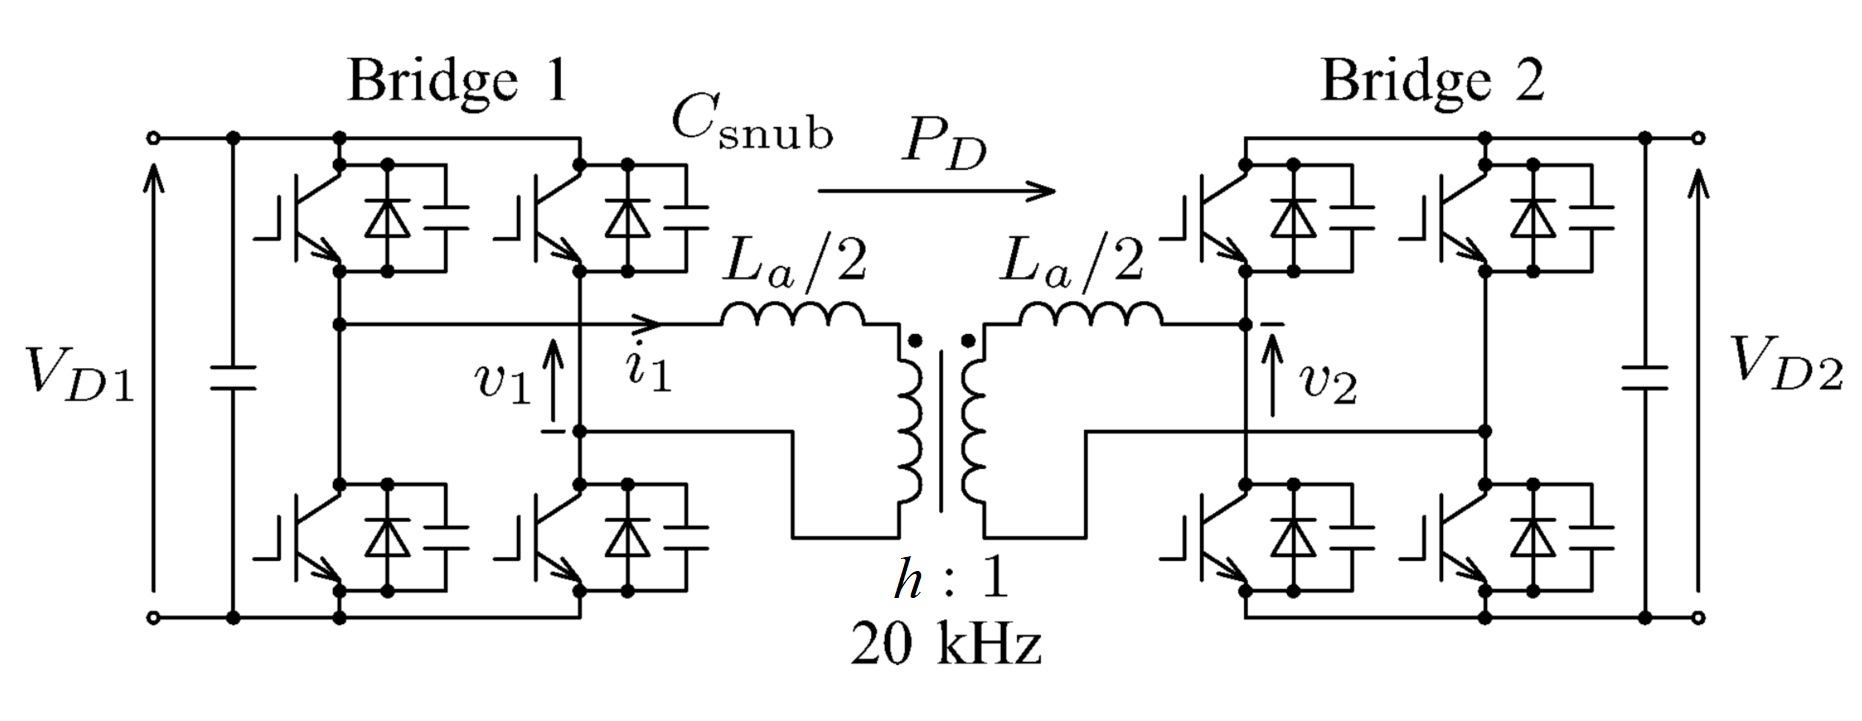
\includegraphics[width=0.7\textwidth]{EMPC_PNG_Pics/DC_DC_galvanic.png}
        \caption{Bidirectional isolated DC-DC converter, where $V_{D1}$, and $V_{D2}$ are the two end's voltage (in- and output depends on the power flow), $v_1$ and $v_2$ are the transformer voltages, $C_{snub}$ are to reduce switching loss and to damp out
over-voltage, and $h$ is the transformer turn ratio.}
        \label{BASICCSR:fig:DCDCGalvanic}
    \end{figure}
		
The principle of operation of the DC-DC converter is very simple. Two active bridges are interfaced through a transformer and are phase shifted from each other to control the amount of power flow from one DC voltage source to the other. This allows a fixed frequency, square-wave mode of operation and utilization of the leakage inductance of the transformer as the main energy transfer element. The power transfer under idealized conditions is defined as:

\begin{equation}
        \begin{array}{rcl}
            P_D&=&\frac{V_{D1}V_{D2}}{\omega L}\left(\delta-\frac{\delta^2}{\pi}\right)\\
        \end{array}
        \label{BASICMPC:equ:DCDC}
    \end{equation}
		
		where $\omega=2\pi f$ is the switching angular frequency of the two single phase full bridge controllers, $L_a$ is the
sum of the transformer leakage inductance.

\subsection{Three-phase buck-type rectifiers}\label{BASICCSR:sec:CSR}

Three-phase controlled rectifiers have a wide range of applications, from small rectifiers to large high-voltage direct-current transmission systems. They are used e.g. at electrochemical processes, many kinds of motor drives, traction equipment, controlled power supplies. In this thesis only force commuted rectifiers are examined, which are built with semiconductors (IGBTs in this case) with gate-turn-off capability. The gate-turn-off capability allows full control of the converter, because valves can be switched ON and OFF whenever is required. This allows the commutation of the valves, hundreds of times in one period that is not possible with line-commutated rectifiers, where IGBTs are switched ON and OFF only once a cycle. This has the following advantages:

\begin{itemize}
\item The current or voltage can be (pulse width) modulated, generating less harmonic contamination.
\item The power factor (ratio of the real and reactive power) can be controlled and even it can be made leading, signifies that the load is capacitive, as the load “supplies” reactive power.
\item They can be built as voltage-source or current-source based on the required application.
\item The reversal of power in switching rectifiers is by reversal of voltage at the DC link. This allows force commutated rectifiers can be implemented for both, reversal of voltage or reversal of current.
\end{itemize}

There are two ways to implement force commutated three phase rectifiers, as a current-source rectifier (Fig.\ref{BASICMPC:fig:CSR}), where power reversal is by DC voltage reversal, and as a voltage-source rectifier (Fig.\ref{BASICMPC:fig:VSR}), where power reversal is is solved by current reversal at the DC link.


\begin{figure}[h]
                \centering
                \begin{subfigure}[b]{0.9\textwidth}
                    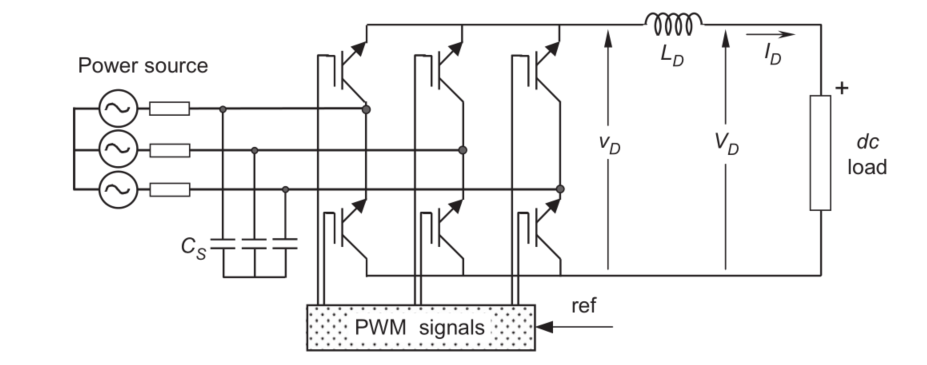
\includegraphics[width=\textwidth]{EMPC_PNG_Pics/BasicCurrentRectifiers.png}
                    \caption{\centering Current source rectifier with capacitive filtering and choke inductance.}
                    \label{BASICMPC:fig:CSR}
                \end{subfigure}
                ~ %add desired spacing between images, e. g. ~, \quad, \qquad, \hfill etc.
                  %(or a blank line to force the subfigure onto a new line)
                \begin{subfigure}[b]{0.9\textwidth}
                    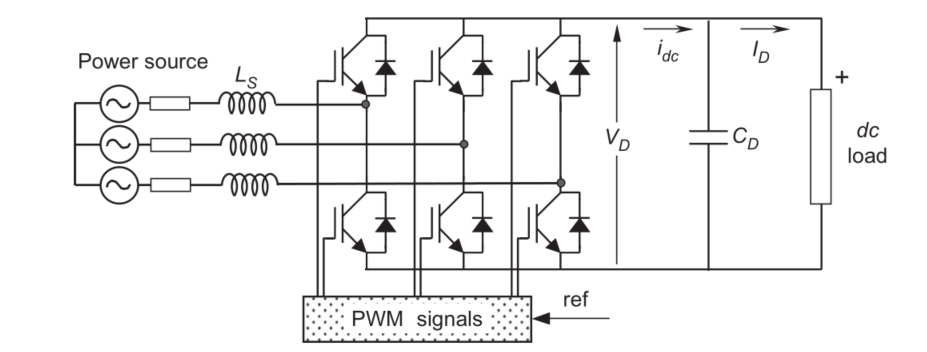
\includegraphics[width=\textwidth]{EMPC_PNG_Pics/BasicVoltageRectifiers.png}
                    \caption{\centering Voltage source rectifier with inductive filtering and DC voltage smoothing capacitance.}
                    \label{BASICMPC:fig:VSR}
                \end{subfigure}
                 %add desired spacing between images, e. g. ~, \quad, \qquad, \hfill etc.
                %(or a blank line to force the subfigure onto a new line)
                %\begin{subfigure}[b]{0.48\textwidth}
                    %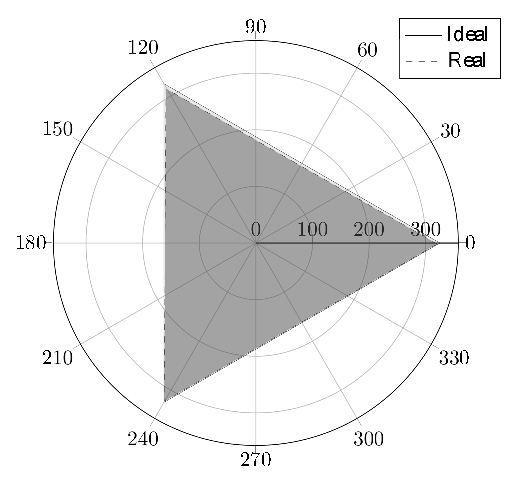
\includegraphics[width=\textwidth]{Unblance_EPS_Pics/EPS_images/square.eps}
                    %\caption{Low correlation with opposed amplitude deviation. The norm values are $G=9322$ and $TDV=0.5198$.}
                    %\label{fig:cases_C}
                %\end{subfigure}
                %~
                %\begin{subfigure}[b]{0.48\textwidth}
                    %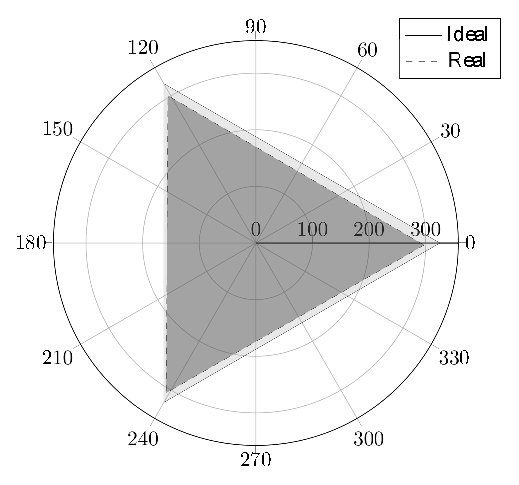
\includegraphics[width=\textwidth]{Unblance_EPS_Pics/EPS_images/circle.eps}
                    %\caption{\centering Low correlation with uniform voltage drop. The norm values are $G=6280$ and $TDV=0.156$.}
                    %\label{fig:cases_D}
                %\end{subfigure}


                \caption{Basic topologies of force commuted rectifiers.}
            \end{figure}

%\begin{figure}[!ht]
        %\centering
        %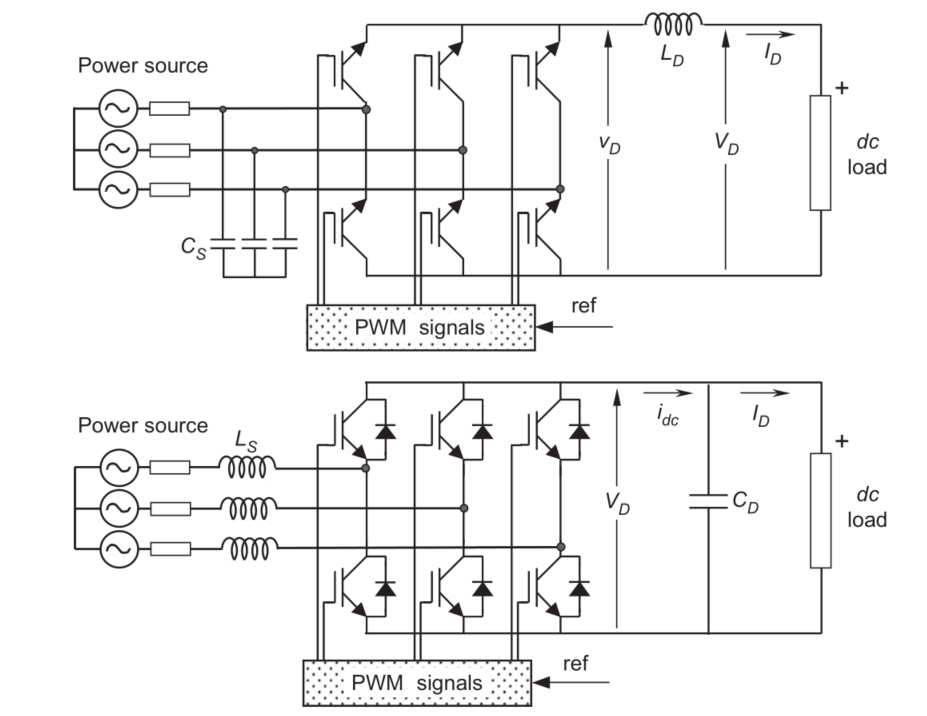
\includegraphics[width=0.9\textwidth]{EMPC_PNG_Pics/CurrentVoltageRectifiers.png}
        %\caption{Basic topologies of force commuted rectifiers.}
        %\label{BASICCSR:fig:topologies}
    %\end{figure}


As  general case be a front-end  converter power supply (e.g. lighting or telecommunications) shall be designed such that it should have approximately these general characteristics: sinusoidal main currents, unity power factor, high power density and simplicity of the power circuit structure. Two structures are most fitted for the task. First a boost-type input rectifier (e.g., Vienna rectifier, \cite{kolar1996design}), that typically features two $400$ V output voltages with a three-level isolated  DC-DC  converter  or  two  isolated  DC-DC  output  stage (see Fig. \ref{EMPC:fig:network} in Ch.5.). The second candidate is the buck-type  input  rectifier (or current source rectifier (CSR))  (conventionally  six-switch topologies as proposed in \cite{zargari1993current}, \cite{sato1993state}) with only one two-level isolated  DC-DC  converter  output  stage.  Also the  input  stage  can be realized as a three-switch topology with considerably  lower  system  complexity  as  compared  to  the boost-type structure. In particular, the number of utilized active and passive components is much lower. Furthermore, there is no middle-point that has to be stabilized, as this is the case for the boost-type structures, making control and active filter design less complex. Further system advantages are the potential of direct start-up and the implicit over current protection in case of an output short circuit. Therefore, these topologies of high interest for many safety critical applications as such future electric aircraft, or automotive applications or as power supplies for process technology \cite{nussbaumer2007comprehensive}.
The three-switch buck rectifier topology was first proposed in \cite{malesani1987three}. In \cite{itoh1989steady} and \cite{tooth2000effects}, aspects of the system modulation and control have been treated. The application of the topology used as an active filter is discussed in \cite{salo2005three}.  The addition of a DC-DC output boost-stage has been proposed in \cite{baumannnew} in order to maintain 400 V output voltage for a wide input voltage range and for the case of unbalanced mains as, e.g., the loss of one phase.

\myparagraph{Basic operation principles}\label{BASICCSR:sec:OperationPrinciple}

For the derivation of the relative on-times of the three buck transistors $S_i$ with the following assumptions are made for clarity and facilitation of calculations:
\begin{itemize}
	\item The AC-side filter capacitor voltages ($v_{c_p}$, where $p\in\{1,2,3\}$) at the input of the CSR are sinusoidal and in phase with the main harmonic component of voltage.
	
	\begin{equation}
        \begin{array}{rcl}
            v_{c_1}&=&\widehat{v}_c\cos(\omega t)\\
						v_{c_2}&=&\widehat{v}_c\cos(\omega t-2\pi/3)\\
						v_{c_3}&=&\widehat{v}_c\cos(\omega t+2\pi/3),\\
        \end{array}
        \label{BASICMPC:equ:phasorvect}
    \end{equation}
	where $\omega$ is the network voltage's angular velocity.
	
	\item The mains currents are assumed to be equal to the fundamental component of the rectifier input currents.
	\item The current in the DC output inductor $L_{D}$ is not affected by the high frequency ripple due to the switching operation.
\end{itemize}

 For achieving ohmic mains behavior also in case of unbalanced fundamental harmonics conditions the explained modulation method can still be utilized, however, additionally the control structure presented in \cite{baumann2005novel} has to be employed.\\
The waveforms of the phase and line-to-line mains voltages are divided into twelve sectors of $\frac{\pi}{6}$ rad wide shown in Fig.\ref{BASICCSR:fig:waves}. The following calculations are based on the analysis of the first sector which is characterized by the voltage harmonic phase relation. For the remaining sectors the calculations can be accomplished in an similar manner \cite{nussbaumer2007comprehensive}.

\begin{figure}[!ht]
        \centering
        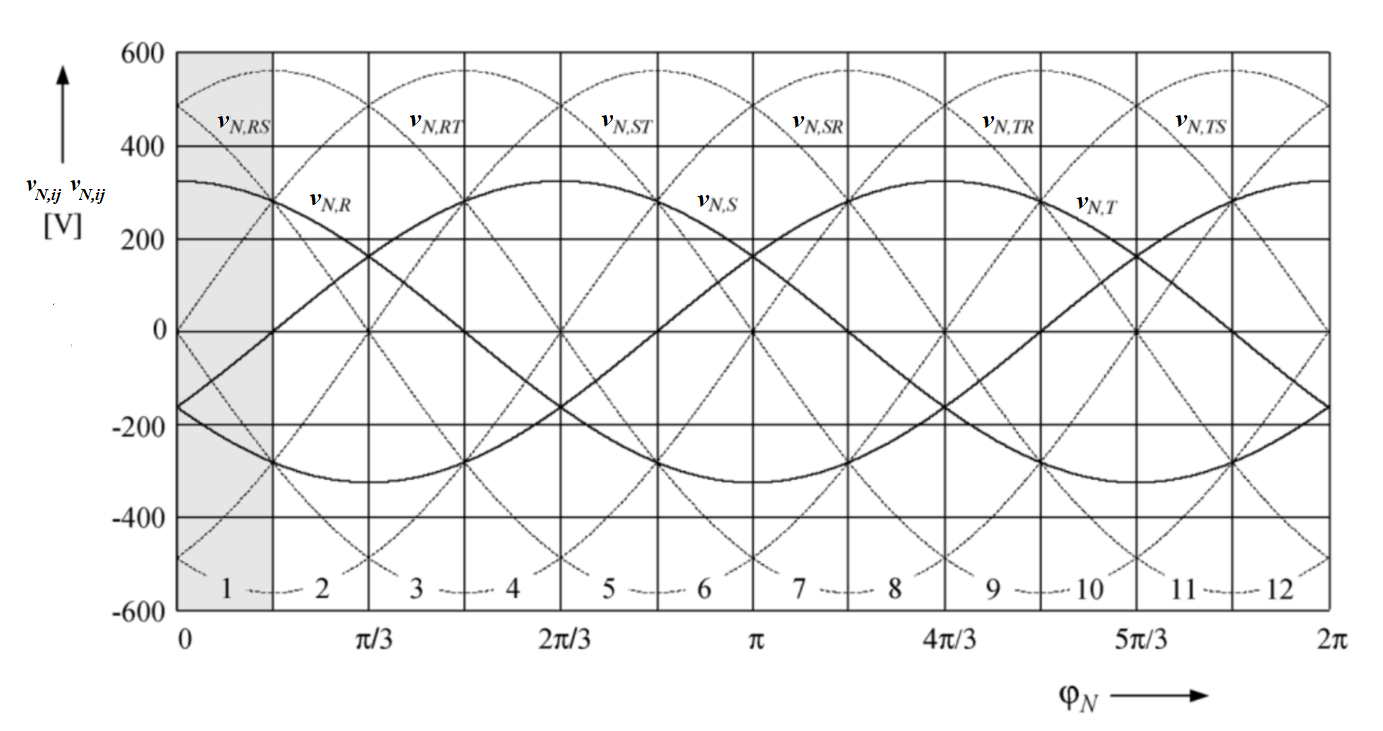
\includegraphics[width=\textwidth]{EMPC_PNG_Pics/Waves.png}
        \caption{Phase voltages $v_{i}$, where line-to-line voltages $v_{N,ij}=v_{N,i}-v_{N,j}$, $(i,j)\in\{R,S,T\}$ and sectors $1$ to $12$ being defined by the different relations of the instantaneous values of the mains phase voltages for $v = 400 V$}
        \label{BASICCSR:fig:waves}
    \end{figure}
		
		Accordingly, on AC side, if conditions are favorable, inductor current can appear in an instant of time either in two out
of three phases or in none. In this modulation technique, the switches in each converter leg can conduct only one at the time (aside from zero states, where both upper and lower switches are conducting). When the upper leg is conducting it is indicated by `$1$', when the lower  `$-1$' and when neither `$0$'. As such the choice whether upper or lower switch of the leg conducts current depends of the reference current vector's sector location.
According to the actual switch combination the DC link current shaped by the choke inductance, and distributed to two of the input phases or the freewheeling diode. With this, the input current space vectors can be calculated for each of the before-mentioned switching states. Generally the space vector of three-phase quantities (e.g., for the rectifier input current) are described as:

\begin{equation}
        \begin{array}{rcl}
            \vec{i}&=&\frac{2}{3}\left(\vec{i}_a+\vec{i}_be^{\frac{j\pi}{3}}+\vec{i}_bc^{\frac{4j\pi}{3}}\right).\\
        \end{array}
        \label{BASICCSR:eqn:currents_all}
    \end{equation}
		
		Based on \ref{BASICCSR:eqn:currents_all} the corresponding active space vectors in the first sector can be obtained as:
		
		\begin{equation}
        \begin{array}{rcl}
            \vec{i}_{(1,0,-1)}=\vec{i}_1&=&2i_{dc}e^{j\pi/6}/\sqrt{3}\\
						\vec{i}_{(0,1,-1)}=\vec{i}_2&=&2i_{dc}e^{j\pi/2}/\sqrt{3}\\
						\vec{i}_{(-1,1,0)}=\vec{i}_3&=&2i_{dc}e^{j5\pi/6}/\sqrt{3}\\
        \end{array}
        \label{BASICCSR:eqn:currents}
    \end{equation}
		
		The resulting discrete space vectors can be used to synthesize desired current
space vector $\vec{i}_{ref}$.

The modulation methods were evaluated in and chosen for this paper based on \cite{moussaoui2005open}, which ensures minimum switching-losses, minimum ripple values of the input capacitor voltages and of the output inductor current. According to this modulation, each pulse interval comprises two active states and a freewheeling state, arranged symmetrically about the middle of the pulse interval (see Table \ref{EMPC:tbl:sequence}). For more in depth functional description see section \ref{EMPC:sec:Modulation}.

\subsection{Coordinate transformations}

In section \ref{EMPC:sec:ModelofCSR} the three phase current source rectifier's (CSR) equations are converted to different coordinate spaces.

\subsubsection{Clarke transformation}\label{BASICCSR:sec:Clarke}

In electrical engineering, Clarke transformation is a mathematical transformation employed to simplify the analysis of three-phase circuits. Conceptually it is similar to the Park transformation. One very useful application is the generation of the reference signal used for space vector modulation control of three-phase inverters. The transformation follows:

\begin{equation}
        \begin{array}{rcl}
            \textbf{i}_{\alpha\beta\gamma}(t)&=&T_{Clarke}\textbf{i}_{abc}(t)
            \begin{bmatrix}
            1& -\frac{1}{2}& -\frac{1}{2}\\
            0& \frac{\sqrt{3}}{2}& -\frac{\sqrt{3}}{2}\\
            \frac{1}{2}& \frac{1}{2}& \frac{1}{2}\\
            \end{bmatrix}
            \begin{bmatrix}
            i_a(t)\\
            i_b(t)\\
            i_c(t)\\
            \end{bmatrix},
        \end{array}
        \label{BASICCSR:eqn:Clarke}
    \end{equation}

    where $\textbf{i}_{abc}$ is the generic three phase current sequence, and $\textbf{i}_{\alpha\beta\gamma}$ is given by the transformation.

    \subsubsection{Park transformation}\label{BASICCSR:sec:Park}

The Park transformation is a tensor that rotates the reference frame of a three-element vector or a three-by-three element matrix in an effort to simplify analysis. The transform can be used to rotate the reference frames of AC waveforms such that they become DC signals. Simplified calculations can then be carried out on these dc quantities before performing the inverse transform to recover the actual three-phase ac results. As an example, the Park transform is often used in order to simplify the analysis of three-phase synchronous machines or to simplify calculations for the control of three-phase inverters. In analysis of three-phase synchronous machines the transformation transfers three-phase stator and rotor quantities into a single rotating reference frame to eliminate the effect of time-varying inductances. The transformation follows:


\begin{equation}
        \begin{array}{rcl}
            \textbf{i}_{dq0}(t)&=&T_{Park}\textbf{i}_{abc}(t)
            \sqrt{\frac{2}{3}}\begin{bmatrix}
            \cos(\theta)& \cos(\theta-\frac{2\pi}{3})& \cos(\theta+\frac{2\pi}{3})\\
            -\sin(\theta)& -\sin(\theta-\frac{2\pi}{3})& -\sin(\theta+\frac{2\pi}{3})\\
            \frac{\sqrt{2}}{2}& \frac{\sqrt{2}}{2}& \frac{\sqrt{2}}{2}\\
            \end{bmatrix}
            \begin{bmatrix}
            i_a(t)\\
            i_b(t)\\
            i_c(t)\\
            \end{bmatrix},
        \end{array}
        \label{BASICCSR:eqn:Park}
    \end{equation}

    where $\theta$ is instantaneous angular position of an arbitrary frequency.
